% ============================================================
% Introduction to Git for Code
% Beamer slide deck — UP EBIT Template
% ============================================================
\documentclass[aspectratio=169, 11pt]{beamer}

% --- UP EBIT Theme ------------------------------------------
\usepackage{beamerthemeUP}

% --- Packages -----------------------------------------------
\usepackage[utf8]{inputenc}
\usepackage[T1]{fontenc}
\usepackage{lmodern}
\usepackage{booktabs}
\usepackage{hyperref}
\usepackage{listings}
\usetikzlibrary{shapes, arrows.meta, positioning, fit}

% --- Code listing style -------------------------------------
\lstdefinestyle{terminal}{
  basicstyle=\ttfamily\scriptsize,
  keywordstyle=\color{UPBlue}\bfseries,
  commentstyle=\color{gray},
  stringstyle=\color{EBITTeal},
  backgroundcolor=\color{black!5},
  frame=single,
  rulecolor=\color{black!20},
  breaklines=true,
  columns=fullflexible,
  keepspaces=true,
  showstringspaces=false,
  tabsize=2,
}
\lstset{style=terminal}

% ============================================================
\begin{document}

% ------ Title -----------------------------------------------
\uptitleframe{Introduction to\\Git for Code}{Dr Muaaz Bhamjee\\[0.15cm]{\small Department of Mechanical \& Aeronautical Engineering}}

% ------ Outline ---------------------------------------------
{
\setbeamertemplate{background}{}% clean outline slide
\begin{frame}{Outline}
  \tableofcontents
\end{frame}
}

% ============================================================
\section{Why Version Control?}
% ============================================================

\begin{frame}{The Problem}
  \begin{columns}[T]
    \begin{column}{0.48\textwidth}
      \textbf{Without version control:}
      \begin{itemize}
        \item \texttt{solver\_v1.py}
        \item \texttt{solver\_v2\_fixed.py}
        \item \texttt{solver\_FINAL.py}
        \item \texttt{solver\_FINAL\_actually.py}
        \item ``Who changed line 47 and why?''
        \item ``It worked yesterday\ldots''
      \end{itemize}
    \end{column}
    \begin{column}{0.48\textwidth}
      \textbf{With Git:}
      \begin{itemize}
        \item One file: \texttt{solver.py}
        \item Every change recorded with context
        \item Revert to any point in history
        \item Multiple people, zero overwrites
        \item Experiment safely in branches
        \item Automated testing on every push
      \end{itemize}
    \end{column}
  \end{columns}
\end{frame}

\begin{frame}{Git --- The Big Picture}
  \begin{itemize}
    \item \textbf{Distributed} version control --- every clone is a full backup.
    \item Created by Linus Torvalds (2005) for Linux kernel development.
    \item De facto standard: used by virtually every open-source and industry project.
  \end{itemize}

  \vspace{0.5em}
  \textbf{Four ways to use Git (all talk to the same repo):}
  \begin{enumerate}
    \item \textbf{Terminal} --- \texttt{git} commands (maximum power)
    \item \textbf{GitHub UI} --- web browser (quick edits, reviews)
    \item \textbf{GitHub CLI} --- \texttt{gh} commands (GitHub features in terminal)
    \item \textbf{VS Code} --- Source Control panel (visual, integrated)
  \end{enumerate}

  \vspace{0.5em}
  \begin{alertblock}{Hosting platforms}
    We use \textbf{GitHub} in this lecture. \textbf{GitLab} and \textbf{Bitbucket} are popular alternatives --- the Git commands are identical; only the web UI and CI features differ.
  \end{alertblock}
\end{frame}

% ============================================================
\section{Installation \& Setup}
% ============================================================

\begin{frame}[fragile]{Installing Git}
  \begin{columns}[T]
    \begin{column}{0.48\textwidth}
      \textbf{Windows:}
      \begin{itemize}
        \item Download from \url{https://git-scm.com}
        \item Includes \textbf{Git Bash} (Linux-like terminal)
        \item Or: \texttt{winget install Git.Git}
      \end{itemize}

      \vspace{0.5em}
      \textbf{macOS:}
      \begin{itemize}
        \item Xcode tools: \texttt{xcode-select --install}
        \item Or: \texttt{brew install git}
      \end{itemize}
    \end{column}
    \begin{column}{0.48\textwidth}
      \textbf{Linux (Debian/Ubuntu):}
      \begin{lstlisting}[language=bash]
sudo apt update
sudo apt install git
      \end{lstlisting}

      \vspace{0.5em}
      \textbf{Verify:}
      \begin{lstlisting}[language=bash]
git --version
# git version 2.43.0
      \end{lstlisting}
    \end{column}
  \end{columns}
\end{frame}

\begin{frame}[fragile]{First-Time Configuration}
  These settings are stored in \texttt{\textasciitilde/.gitconfig} and apply to all repos.

  \begin{lstlisting}[language=bash]
# Identity (required --- used in every commit)
git config --global user.name "Muaaz Bhamjee"
git config --global user.email "muaaz.bhamjee@up.ac.za"

# Default branch name
git config --global init.defaultBranch main

# Preferred editor (for commit messages)
git config --global core.editor "code --wait"   # VS Code
# git config --global core.editor "nano"         # alternative

# Line endings (important for cross-platform teams)
git config --global core.autocrlf input          # macOS / Linux
# git config --global core.autocrlf true         # Windows

# Verify
git config --list
  \end{lstlisting}
\end{frame}

\begin{frame}[fragile]{Installing the GitHub CLI (\texttt{gh})}
  \begin{columns}[T]
    \begin{column}{0.48\textwidth}
      \textbf{Windows:}
      \begin{lstlisting}[language=bash]
winget install GitHub.cli
      \end{lstlisting}

      \textbf{macOS:}
      \begin{lstlisting}[language=bash]
brew install gh
      \end{lstlisting}

      \textbf{Linux:}
      \begin{lstlisting}[language=bash]
sudo apt install gh
# or: snap install gh
      \end{lstlisting}
    \end{column}
    \begin{column}{0.48\textwidth}
      \textbf{Verify:}
      \begin{lstlisting}[language=bash]
gh --version
# gh version 2.x.x
      \end{lstlisting}

      \vspace{0.5em}
      \texttt{gh} is \textbf{not} a replacement for \texttt{git} --- it adds
      GitHub-specific features (PRs, issues, releases, auth) on top of Git.
    \end{column}
  \end{columns}
\end{frame}

% ============================================================
\section{Authentication}
% ============================================================

\begin{frame}{Authentication Overview}
  To push code to GitHub you must prove you are who you claim to be.

  \vspace{0.5em}
  \begin{table}
    \centering
    \begin{tabular}{@{} l l l @{}}
      \toprule
      \textbf{Method} & \textbf{How it works} & \textbf{Best for} \\
      \midrule
      SSH key       & Public/private key pair & Daily use (recommended) \\
      HTTPS + \texttt{gh auth} & OAuth via browser & Quick start \\
      Personal Access Token & Token string      & CI/CD, scripts, API \\
      \bottomrule
    \end{tabular}
  \end{table}

  \vspace{0.5em}
  \begin{block}{Key point}
    GitHub \textbf{removed password authentication} for Git operations in 2021.
    You \emph{must} use one of the methods above.
  \end{block}
\end{frame}

\begin{frame}[fragile]{Option 1: SSH Key (Recommended)}
  \textbf{Step 1 --- Generate a key pair:}
  \begin{lstlisting}[language=bash]
ssh-keygen -t ed25519 -C "muaaz.bhamjee@up.ac.za"
# Accept default path: ~/.ssh/id_ed25519
# Set a passphrase (or leave blank)
  \end{lstlisting}

  \textbf{Step 2 --- Add the public key to GitHub:}
  \begin{lstlisting}[language=bash]
# Copy the public key to clipboard
cat ~/.ssh/id_ed25519.pub
# (macOS: pbcopy < ~/.ssh/id_ed25519.pub)
# (Windows Git Bash: clip < ~/.ssh/id_ed25519.pub)
  \end{lstlisting}
  Then: GitHub $\to$ Settings $\to$ SSH and GPG keys $\to$ \textbf{New SSH key} $\to$ paste.

  \vspace{0.3em}
  \textbf{Step 3 --- Test the connection:}
  \begin{lstlisting}[language=bash]
ssh -T git@github.com
# "Hi username! You've successfully authenticated..."
  \end{lstlisting}

  \textbf{Step 4 --- Clone with SSH URL:}
  \begin{lstlisting}[language=bash]
git clone git@github.com:username/repo.git
  \end{lstlisting}
\end{frame}

\begin{frame}[fragile]{Option 2: HTTPS via \texttt{gh auth login}}
  The simplest way to authenticate --- \texttt{gh} handles everything.

  \begin{lstlisting}[language=bash]
gh auth login
  \end{lstlisting}

  Follow the interactive prompts:
  \begin{enumerate}
    \item Account: \textbf{GitHub.com}
    \item Protocol: \textbf{HTTPS}
    \item Authenticate: \textbf{Login with a web browser}
    \item Copy the one-time code, press Enter
    \item Paste the code in the browser and authorise
  \end{enumerate}

  \vspace{0.3em}
  \begin{lstlisting}[language=bash]
# Verify
gh auth status
# github.com: Logged in as username

# gh also configures git's credential helper automatically
git clone https://github.com/username/repo.git   # works!
  \end{lstlisting}

  \begin{block}{Tip}
    \texttt{gh auth login} also sets up Git credential caching, so regular \texttt{git push} over HTTPS will work without re-entering credentials.
  \end{block}
\end{frame}

\begin{frame}[fragile]{Option 3: Personal Access Token (PAT)}
  For scripts, CI/CD pipelines, and API access.

  \vspace{0.3em}
  \textbf{Generate a token:}
  \begin{enumerate}
    \item GitHub $\to$ Settings $\to$ Developer settings $\to$ \textbf{Personal access tokens} $\to$ \textbf{Fine-grained tokens} (recommended).
    \item Select scopes: \texttt{repo}, \texttt{workflow} (as needed).
    \item Copy the token --- you will not see it again.
  \end{enumerate}

  \textbf{Use with Git:}
  \begin{lstlisting}[language=bash]
# When prompted for password, paste the token instead
git clone https://github.com/username/private-repo.git
Username: your-username
Password: ghp_xxxxxxxxxxxxxxxxxxxx   # <-- paste token here
  \end{lstlisting}

  \textbf{Or with \texttt{gh}:}
  \begin{lstlisting}[language=bash]
echo "ghp_xxxxxxxxxxxxxxxxxxxx" | gh auth login --with-token
  \end{lstlisting}

  \begin{alertblock}{Security}
    Never commit tokens to a repository. Use environment variables or a secrets manager.
  \end{alertblock}
\end{frame}

\begin{frame}[fragile]{SSH vs HTTPS --- Which URL?}
  \begin{table}
    \centering
    \begin{tabular}{@{} l l l @{}}
      \toprule
      & \textbf{SSH} & \textbf{HTTPS} \\
      \midrule
      URL format & \texttt{git@github.com:user/repo.git} & \texttt{https://github.com/user/repo.git} \\
      Auth       & Key pair (no password)       & Token / \texttt{gh auth} \\
      Firewall   & Port 22 (sometimes blocked)  & Port 443 (always open) \\
      Setup      & One-time key generation       & \texttt{gh auth login} \\
      \bottomrule
    \end{tabular}
  \end{table}

  \vspace{0.5em}
  \textbf{Switching an existing repo:}
  \begin{lstlisting}[language=bash]
# Check current remote
git remote -v

# Switch from HTTPS to SSH
git remote set-url origin git@github.com:user/repo.git

# Switch from SSH to HTTPS
git remote set-url origin https://github.com/user/repo.git
  \end{lstlisting}
\end{frame}

% ============================================================
\section{Git via the Terminal}
% ============================================================

\begin{frame}[fragile]{Core Concepts}
  \begin{center}
    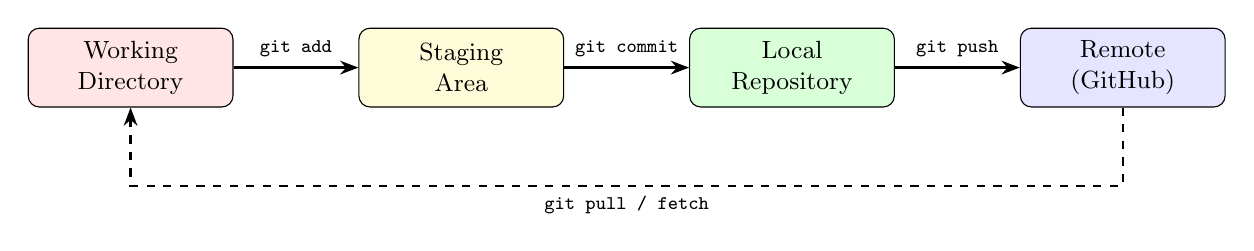
\begin{tikzpicture}[
      box/.style={draw, rounded corners, minimum width=2.6cm, minimum height=1cm, align=center, font=\small},
      arr/.style={->, thick, >=Stealth}
    ]
      \node[box, fill=red!10]    (wd)     at (0,0)     {Working\\Directory};
      \node[box, fill=yellow!15] (sa)     at (4.2,0)   {Staging\\Area};
      \node[box, fill=green!15]  (local)  at (8.4,0)   {Local\\Repository};
      \node[box, fill=blue!10]   (remote) at (12.6,0)  {Remote\\(GitHub)};

      \draw[arr] (wd)    -- node[above, font=\ttfamily\scriptsize] {git add} (sa);
      \draw[arr] (sa)    -- node[above, font=\ttfamily\scriptsize] {git commit} (local);
      \draw[arr] (local) -- node[above, font=\ttfamily\scriptsize] {git push} (remote);
      \draw[arr, dashed] (remote) -- ++(0,-1.5) -| node[below, near start, font=\ttfamily\scriptsize] {git pull / fetch} (wd);
    \end{tikzpicture}
  \end{center}

  \vspace{0.3em}
  \begin{itemize}
    \item \textbf{Working directory} --- your files on disk.
    \item \textbf{Staging area} (index) --- changes selected for the next commit.
    \item \textbf{Local repo} (\texttt{.git/}) --- full history on your machine.
    \item \textbf{Remote} --- the copy on GitHub (or GitLab).
  \end{itemize}
\end{frame}

\begin{frame}[fragile]{Creating and Cloning Repos}
  \textbf{New repo from scratch:}
  \begin{lstlisting}[language=bash]
mkdir my-project && cd my-project
git init                        # creates .git/
echo "# My Project" > README.md
git add README.md
git commit -m "Initial commit"
  \end{lstlisting}

  \textbf{Link to GitHub and push:}
  \begin{lstlisting}[language=bash]
# Create the remote repo with gh (one command!)
gh repo create my-project --public --source=. --push
  \end{lstlisting}

  \textbf{Clone an existing repo:}
  \begin{lstlisting}[language=bash]
git clone git@github.com:username/repo.git
cd repo
  \end{lstlisting}
\end{frame}

\begin{frame}[fragile]{The Daily Workflow}
  \begin{lstlisting}[language=bash]
# 1. Check status
git status                     # see what's changed

# 2. Stage changes
git add solver.py              # stage one file
git add .                      # stage everything

# 3. Commit
git commit -m "Fix boundary condition at inlet"

# 4. Push to remote
git push

# 5. Pull latest changes (from collaborators)
git pull
  \end{lstlisting}

  \vspace{0.3em}
  \textbf{Useful inspection commands:}
  \begin{lstlisting}[language=bash]
git log --oneline --graph      # visual commit history
git diff                       # unstaged changes
git diff --staged              # staged changes
git show abc1234               # inspect a specific commit
git blame solver.py            # who changed each line?
  \end{lstlisting}
\end{frame}

\begin{frame}[fragile]{Branching \& Merging}
  Branches let you work on features in isolation.

  \begin{lstlisting}[language=bash]
# Create and switch to a new branch
git checkout -b feature/new-solver

# ... edit files, add, commit ...

# Switch back to main
git checkout main

# Merge the feature branch
git merge feature/new-solver

# Delete the branch (clean up)
git branch -d feature/new-solver
  \end{lstlisting}

  \vspace{0.3em}
  \begin{center}
    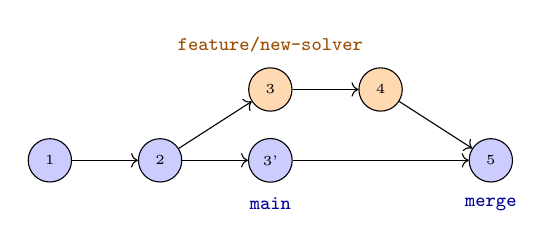
\begin{tikzpicture}[
      c/.style={circle, draw, fill=blue!20, minimum size=0.55cm, font=\tiny},
      f/.style={circle, draw, fill=orange!30, minimum size=0.55cm, font=\tiny},
    ]
      \node[c] (c1) at (0,0)   {1};
      \node[c] (c2) at (1.4,0) {2};
      \node[f] (f1) at (2.8,0.9) {3};
      \node[f] (f2) at (4.2,0.9) {4};
      \node[c] (c3) at (2.8,0)   {3'};
      \node[c] (c4) at (5.6,0)   {5};
      \draw[->] (c1)--(c2); \draw[->] (c2)--(f1); \draw[->] (f1)--(f2);
      \draw[->] (c2)--(c3); \draw[->] (c3)--(c4); \draw[->] (f2)--(c4);
      \node[above=2pt, font=\scriptsize\ttfamily, orange!60!black] at (f1.north) {feature/new-solver};
      \node[below=2pt, font=\scriptsize\ttfamily, blue!60!black] at (c3.south) {main};
      \node[below=2pt, font=\scriptsize\ttfamily, blue!60!black] at (c4.south) {merge};
    \end{tikzpicture}
  \end{center}
\end{frame}

\begin{frame}[fragile]{Handling Merge Conflicts}
  A conflict occurs when two branches change the \textbf{same line(s)}.

  \begin{lstlisting}
<<<<<<< HEAD
velocity = 5.0   # your change on main
=======
velocity = 10.0  # their change on feature branch
>>>>>>> feature/new-solver
  \end{lstlisting}

  \textbf{Resolution steps:}
  \begin{enumerate}
    \item Open the conflicted file.
    \item Choose the correct code (or combine both).
    \item Remove the \texttt{<{}<{}<{}<{}}, \texttt{={}={}={}={}}, \texttt{>{}>{}>{}>{}} markers.
    \item Stage and commit:
  \end{enumerate}

  \begin{lstlisting}[language=bash]
git add solver.py
git commit -m "Resolve merge conflict in solver.py"
  \end{lstlisting}

  \begin{block}{Tip}
    VS Code highlights conflicts with colour and offers \textbf{Accept Current / Incoming / Both} buttons --- much easier than editing markers by hand.
  \end{block}
\end{frame}

\begin{frame}[fragile]{Undoing Things}
  \begin{table}
    \centering
    \begin{tabular}{@{} l l @{}}
      \toprule
      \textbf{Situation} & \textbf{Command} \\
      \midrule
      Unstage a file                & \texttt{git restore --staged file.py} \\
      Discard local changes         & \texttt{git restore file.py} \\
      Amend last commit message     & \texttt{git commit --amend} \\
      Undo last commit (keep files) & \texttt{git reset --soft HEAD\textasciitilde1} \\
      Undo last commit (discard)    & \texttt{git reset --hard HEAD\textasciitilde1} \\
      Revert a pushed commit        & \texttt{git revert abc1234} \\
      \bottomrule
    \end{tabular}
  \end{table}

  \begin{alertblock}{Warning}
    \texttt{git reset --hard} is destructive. Only use it on commits that haven't been pushed, or when you truly want to discard work.
  \end{alertblock}
\end{frame}

\begin{frame}[fragile]{Stashing Work}
  Need to switch branches but have uncommitted changes?

  \begin{lstlisting}[language=bash]
# Save current changes to the stash
git stash

# Do other work, switch branches, etc.
git checkout main
# ...

# Come back and restore
git checkout feature/experiment
git stash pop                  # apply and remove from stash
  \end{lstlisting}

  \vspace{0.3em}
  \begin{lstlisting}[language=bash]
git stash list                 # see all stashed changes
git stash apply stash@{0}     # apply without removing
git stash drop stash@{0}      # discard a stash entry
  \end{lstlisting}
\end{frame}

% ============================================================
\section{Git via the GitHub UI}
% ============================================================

\begin{frame}{GitHub Web Interface}
  \textbf{What you can do from github.com:}
  \begin{itemize}
    \item \textbf{Browse} code, commit history, branches, and diffs.
    \item \textbf{Edit} files directly (pencil icon) --- good for quick fixes.
    \item \textbf{Create / review pull requests} --- the core collaboration tool.
    \item \textbf{Manage issues} --- bug tracking, feature requests, task boards.
    \item \textbf{Releases \& tags} --- publish versions.
    \item \textbf{Actions} --- CI/CD pipelines (automated testing, deployment).
    \item \textbf{Settings} --- branch protection, collaborators, webhooks.
  \end{itemize}

  \vspace{0.5em}
  \begin{block}{When to use the UI}
    Quick documentation edits, reviewing pull requests, managing issues, and project boards. For actual coding, use a local tool.
  \end{block}
\end{frame}

\begin{frame}{Pull Requests --- The Collaboration Workflow}
  A \textbf{pull request} (PR) proposes merging one branch into another.

  \vspace{0.3em}
  \textbf{Typical flow:}
  \begin{enumerate}
    \item Create a feature branch and push it.
    \item Open a PR on GitHub (or with \texttt{gh pr create}).
    \item Team reviews: comments, suggestions, approvals.
    \item CI tests run automatically (if configured).
    \item Merge the PR (squash, merge commit, or rebase).
    \item Delete the feature branch.
  \end{enumerate}

  \vspace{0.5em}
  \begin{center}
    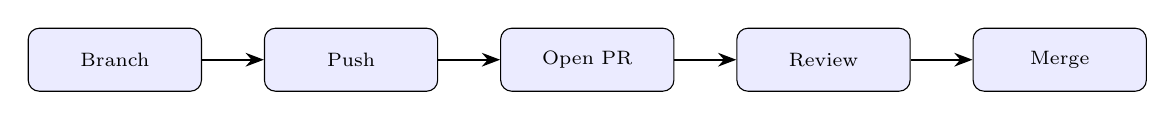
\begin{tikzpicture}[
      box/.style={draw, rounded corners, fill=blue!8, minimum width=2.2cm, minimum height=0.8cm, align=center, font=\scriptsize},
      arr/.style={->, thick, >=Stealth}
    ]
      \node[box] (branch) at (0,0)    {Branch};
      \node[box] (push)   at (3,0)    {Push};
      \node[box] (pr)     at (6,0)    {Open PR};
      \node[box] (review) at (9,0)    {Review};
      \node[box] (merge)  at (12,0)   {Merge};
      \draw[arr] (branch)--(push);
      \draw[arr] (push)--(pr);
      \draw[arr] (pr)--(review);
      \draw[arr] (review)--(merge);
    \end{tikzpicture}
  \end{center}
\end{frame}

% ============================================================
\section{Git via the GitHub CLI (\texttt{gh})}
% ============================================================

\begin{frame}[fragile]{\texttt{gh} --- GitHub from Your Terminal}
  The GitHub CLI brings PRs, issues, repos, and auth to the command line.

  \begin{lstlisting}[language=bash]
# Authenticate (first time)
gh auth login

# Create a repo
gh repo create my-solver --public --clone

# Create a pull request
gh pr create --title "Add turbulence model" --body "Implements k-epsilon"

# List open PRs
gh pr list

# Review & merge a PR
gh pr view 42
gh pr merge 42 --squash
  \end{lstlisting}
\end{frame}

\begin{frame}[fragile]{\texttt{gh} --- Issues \& More}
  \begin{lstlisting}[language=bash]
# Create an issue
gh issue create --title "Bug: NaN at boundary" --label "bug"

# List issues
gh issue list

# Close an issue
gh issue close 7

# View repo in browser
gh repo view --web

# Fork a repo
gh repo fork upstream/cool-project --clone

# Create a release
gh release create v1.0.0 --title "First release" --notes "Initial"
  \end{lstlisting}

  \vspace{0.3em}
  \begin{block}{Power user tip}
    Combine \texttt{gh} with shell scripts to automate your workflow, e.g.\ create a PR from a branch with one command alias.
  \end{block}
\end{frame}

% ============================================================
\section{Git via VS Code}
% ============================================================

\begin{frame}{VS Code --- Integrated Git}
  VS Code has \textbf{built-in Git support} --- no extension needed for basics.

  \vspace{0.5em}
  \textbf{Source Control panel} (Ctrl+Shift+G / Cmd+Shift+G):
  \begin{itemize}
    \item See changed files, staged files, and diffs side by side.
    \item Stage/unstage with a single click (\textbf{+} / \textbf{--}).
    \item Write commit messages and commit from the UI.
    \item Push, pull, and sync from the status bar.
    \item Switch branches from the bottom-left corner.
  \end{itemize}

  \vspace{0.5em}
  \textbf{Recommended extension: GitLens}
  \begin{itemize}
    \item Inline blame annotations (who changed this line).
    \item File and line history.
    \item Interactive rebase editor.
    \item Visual commit graph.
    \item Install: Extensions panel $\to$ search ``GitLens'' $\to$ Install.
  \end{itemize}
\end{frame}

\begin{frame}{VS Code Git Workflow --- Step by Step}
  \begin{enumerate}
    \item \textbf{Open a repo:} File $\to$ Open Folder (pick your cloned repo).
    \item \textbf{Edit files} --- modified files appear in Source Control with an \textbf{M}.
    \item \textbf{View diffs:} Click any changed file to see a side-by-side diff.
    \item \textbf{Stage:} Click \textbf{+} next to each file (or \textbf{+} at the top for all).
    \item \textbf{Commit:} Type a message in the text box, press Ctrl+Enter.
    \item \textbf{Push:} Click the sync icon in the status bar, or \textbf{\ldots} $\to$ Push.
    \item \textbf{Pull:} Same sync icon, or \textbf{\ldots} $\to$ Pull.
  \end{enumerate}

  \vspace{0.5em}
  \textbf{Branching in VS Code:}
  \begin{itemize}
    \item Bottom-left shows current branch --- click to switch or create.
    \item Command Palette (Ctrl+Shift+P): \texttt{Git: Create Branch}.
    \item Merge: \texttt{Git: Merge Branch\ldots} from the Command Palette.
  \end{itemize}
\end{frame}

\begin{frame}{VS Code --- Resolving Conflicts Visually}
  When a merge conflict occurs, VS Code:
  \begin{enumerate}
    \item Highlights conflicted regions in \textcolor{green!60!black}{green} (current) and \textcolor{blue!70!black}{blue} (incoming).
    \item Shows inline buttons:
    \begin{itemize}
      \item \textbf{Accept Current Change}
      \item \textbf{Accept Incoming Change}
      \item \textbf{Accept Both Changes}
      \item \textbf{Compare Changes}
    \end{itemize}
    \item After resolving, stage the file and commit.
  \end{enumerate}

  \vspace{0.5em}
  \begin{block}{Three-way merge editor (VS Code 1.69+)}
    For complex conflicts: right-click the file $\to$ \textbf{Open in Merge Editor}. Shows base, current, and incoming side by side with a result pane at the bottom.
  \end{block}
\end{frame}

\begin{frame}{VS Code --- Useful Extensions for Git}
  \begin{table}
    \centering
    \begin{tabular}{@{} l l @{}}
      \toprule
      \textbf{Extension} & \textbf{What it adds} \\
      \midrule
      GitLens              & Blame, history, graph, stash UI \\
      GitHub Pull Requests & Review PRs inside VS Code \\
      Git Graph            & Interactive commit graph \\
      GitHub Copilot       & AI-assisted code (and commit messages) \\
      \bottomrule
    \end{tabular}
  \end{table}

  \vspace{0.5em}
  \textbf{Terminal in VS Code:}\\
  Ctrl+\textasciigrave{} (backtick) opens the integrated terminal --- run \texttt{git} and \texttt{gh} commands without leaving the editor.
\end{frame}

% ============================================================
\section{Branching --- Why \& How}
% ============================================================

\begin{frame}{Why Branch?}
  \begin{columns}[T]
    \begin{column}{0.48\textwidth}
      \textbf{Without branches:}
      \begin{itemize}
        \item Everyone commits to \texttt{main}.
        \item Half-finished features break the code.
        \item ``Who introduced this bug?'' --- hard to isolate.
        \item Rollback means reverting everyone's work.
        \item You're afraid to experiment.
      \end{itemize}
    \end{column}
    \begin{column}{0.48\textwidth}
      \textbf{With branches:}
      \begin{itemize}
        \item \texttt{main} is \textbf{always working}.
        \item Each task lives in its own isolated branch.
        \item Test \& review \emph{before} merging.
        \item Discard a failed experiment = delete a branch.
        \item Multiple people work in parallel, zero interference.
      \end{itemize}
    \end{column}
  \end{columns}

  \vspace{0.5em}
  \begin{alertblock}{Rule \#1}
    \textbf{Never push directly to \texttt{main}.}
    All changes reach \texttt{main} through a pull request. No exceptions.
  \end{alertblock}
\end{frame}

\begin{frame}{Branch Naming Conventions}
  Use a consistent \texttt{type/short-description} format so anyone can tell what a branch is for at a glance.

  \vspace{0.5em}
  \begin{table}
    \centering
    \begin{tabular}{@{} l l l @{}}
      \toprule
      \textbf{Prefix} & \textbf{Purpose} & \textbf{Example} \\
      \midrule
      \texttt{feature/} & New functionality        & \texttt{feature/k-epsilon-model} \\
      \texttt{fix/}     & Bug fix                  & \texttt{fix/inlet-boundary-nan} \\
      \texttt{docs/}    & Documentation only       & \texttt{docs/update-readme} \\
      \texttt{refactor/}& Code restructure         & \texttt{refactor/solver-class} \\
      \texttt{test/}    & Adding / fixing tests    & \texttt{test/mesh-convergence} \\
      \texttt{chore/}   & Tooling, CI, deps        & \texttt{chore/upgrade-numpy} \\
      \texttt{exp/}     & Experimental / throwaway & \texttt{exp/gpu-acceleration} \\
      \bottomrule
    \end{tabular}
  \end{table}

  \vspace{0.5em}
  \textbf{Rules of thumb:}
  \begin{itemize}
    \item Lowercase, hyphens (not underscores or spaces): \texttt{feature/add-solver} \checkmark
    \item Short but descriptive: \texttt{fix/bc} \texttimes \quad \texttt{fix/wall-bc-segfault} \checkmark
    \item Include issue number if applicable: \texttt{fix/42-nan-at-outlet}
  \end{itemize}
\end{frame}

\begin{frame}{The Feature Branch Workflow}
  \begin{enumerate}
    \item \texttt{main} is always deployable / working.
    \item Create a \textbf{feature branch} for each task.
    \item Commit, push, and open a \textbf{pull request}.
    \item Team reviews, CI tests pass, then \textbf{merge}.
    \item Delete the feature branch.
  \end{enumerate}

  \vspace{0.5em}
  \begin{center}
    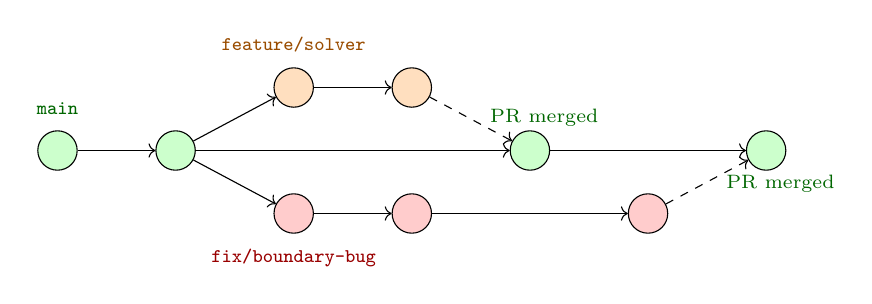
\begin{tikzpicture}[
      c/.style={circle, draw, fill=green!20, minimum size=0.5cm, font=\tiny},
      f/.style={circle, draw, fill=orange!25, minimum size=0.5cm, font=\tiny},
      h/.style={circle, draw, fill=red!20, minimum size=0.5cm, font=\tiny},
    ]
      \node[c] (m1) at (0,0) {};
      \node[c] (m2) at (1.5,0) {};
      \node[c] (m3) at (6,0) {};
      \node[c] (m4) at (9,0) {};
      \node[f] (f1) at (3, 0.8) {};
      \node[f] (f2) at (4.5, 0.8) {};
      \node[h] (h1) at (3, -0.8) {};
      \node[h] (h2) at (4.5, -0.8) {};
      \node[h] (h3) at (7.5, -0.8) {};
      \draw[->] (m1)--(m2); \draw[->] (m2)--(m3); \draw[->] (m3)--(m4);
      \draw[->] (m2)--(f1); \draw[->] (f1)--(f2); \draw[->, dashed] (f2)--(m3);
      \draw[->] (m2)--(h1); \draw[->] (h1)--(h2); \draw[->] (h2)--(h3); \draw[->, dashed] (h3)--(m4);
      \node[above=2pt, font=\scriptsize\ttfamily, orange!60!black] at (f1.north) {feature/solver};
      \node[below=2pt, font=\scriptsize\ttfamily, red!60!black] at (h1.south) {fix/boundary-bug};
      \node[above=2pt, font=\scriptsize\ttfamily, green!40!black] at (m1.north) {main};
      \node[above=0pt, font=\scriptsize, green!40!black] at (m3.north east) {PR merged};
      \node[below=0pt, font=\scriptsize, green!40!black] at (m4.south east) {PR merged};
    \end{tikzpicture}
  \end{center}

  \vspace{0.3em}
  Dashed arrows = \textbf{pull request merge}. No direct commits to \texttt{main}.
\end{frame}

% ============================================================
\section{Forking --- Why \& When}
% ============================================================

\begin{frame}{Branching vs Forking}
  \begin{columns}[T]
    \begin{column}{0.48\textwidth}
      \textbf{Branching}
      \begin{itemize}
        \item Works \emph{within} a single repository.
        \item You need \textbf{write access} (collaborator).
        \item Used by teams that trust each other.
        \item Best for: your own projects, lab group repos, company code.
      \end{itemize}

      \vspace{0.5em}
      \centering
      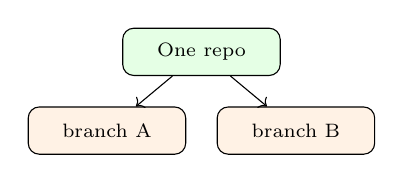
\begin{tikzpicture}[
        box/.style={draw, rounded corners, fill=green!10, minimum width=2cm, minimum height=0.6cm, font=\scriptsize, align=center}
      ]
        \node[box] (repo) at (0,0) {One repo};
        \node[box, fill=orange!10] (b1) at (-1.2,-1) {branch A};
        \node[box, fill=orange!10] (b2) at (1.2,-1) {branch B};
        \draw[->] (repo)--(b1); \draw[->] (repo)--(b2);
      \end{tikzpicture}
    \end{column}
    \begin{column}{0.48\textwidth}
      \textbf{Forking}
      \begin{itemize}
        \item Creates your own \textbf{copy} of the entire repo on GitHub.
        \item You do \textbf{not} need write access to the original.
        \item Used for open-source contributions.
        \item Best for: contributing to projects you don't own.
      \end{itemize}

      \vspace{0.5em}
      \centering
      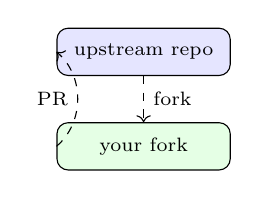
\begin{tikzpicture}[
        box/.style={draw, rounded corners, minimum width=2.2cm, minimum height=0.6cm, font=\scriptsize, align=center}
      ]
        \node[box, fill=blue!10] (upstream) at (0,0) {upstream repo};
        \node[box, fill=green!10] (fork) at (0,-1.2) {your fork};
        \draw[->, dashed] (upstream)--(fork) node[midway, right, font=\scriptsize] {fork};
        \draw[->, dashed] (fork.west) to[bend right=50] node[left, font=\scriptsize] {PR} (upstream.west);
      \end{tikzpicture}
    \end{column}
  \end{columns}
\end{frame}

\begin{frame}[fragile]{The Fork \& Pull Request Workflow}
  \textbf{When to fork:}
  \begin{itemize}
    \item You want to contribute to a repo you \textbf{don't own} (open source, another lab's code).
    \item You want to experiment with someone else's code without affecting the original.
    \item The maintainer hasn't added you as a collaborator.
  \end{itemize}

  \vspace{0.3em}
  \textbf{Steps:}
  \begin{enumerate}
    \item \textbf{Fork} on GitHub (or \texttt{gh repo fork owner/repo --clone}).
    \item Clone \emph{your fork} locally.
    \item Create a feature branch (yes, even in a fork --- never commit to \texttt{main}).
    \item Push to \emph{your fork}.
    \item Open a PR from your fork $\to$ the \textbf{upstream} repo.
    \item Maintainer reviews and merges.
  \end{enumerate}

  \vspace{0.3em}
  \textbf{Keeping your fork in sync:}
  \begin{lstlisting}[language=bash]
git remote add upstream git@github.com:original-owner/repo.git
git fetch upstream
git checkout main
git merge upstream/main
git push origin main           # update your fork on GitHub
  \end{lstlisting}
\end{frame}

\begin{frame}{When to Branch vs Fork --- Quick Guide}
  \begin{table}
    \centering
    \begin{tabular}{@{} l c c @{}}
      \toprule
      \textbf{Scenario} & \textbf{Branch} & \textbf{Fork} \\
      \midrule
      Your own project                    & \checkmark &            \\
      Lab / research group repo           & \checkmark &            \\
      Open-source project (not a member)  &            & \checkmark \\
      Colleague's repo (no write access)  &            & \checkmark \\
      Company repo (you're a collaborator)& \checkmark &            \\
      Want to heavily customise a library &            & \checkmark \\
      \bottomrule
    \end{tabular}
  \end{table}

  \vspace{0.5em}
  \begin{block}{Key insight}
    Forking and branching are not competing strategies --- they complement each other. Even in a fork, you create feature branches and submit PRs. The fork just gives you your own copy to push to.
  \end{block}
\end{frame}

% ============================================================
\section{Pull Requests --- Best Practices}
% ============================================================

\begin{frame}{Why Pull Requests?}
  A pull request (PR) is not just a merge button --- it's a \textbf{quality gate}.

  \vspace{0.5em}
  \textbf{What a PR gives you:}
  \begin{itemize}
    \item \textbf{Code review} --- a second pair of eyes catches bugs, style issues, and design problems.
    \item \textbf{Discussion} --- comments, suggestions, questions, all linked to specific lines.
    \item \textbf{Automated checks} --- CI runs tests, linters, formatters before merge.
    \item \textbf{Audit trail} --- who approved what, when, and why.
    \item \textbf{Knowledge sharing} --- reviewers learn the codebase; authors learn better patterns.
  \end{itemize}

  \vspace{0.5em}
  \begin{alertblock}{Rule \#2}
    \textbf{All changes to \texttt{main} must go through a pull request.}
    Even if you're the only person on the project --- review your own PR, run CI, then merge.
  \end{alertblock}
\end{frame}

\begin{frame}{Writing a Good Pull Request}
  \begin{columns}[T]
    \begin{column}{0.48\textwidth}
      \textbf{PR title:}
      \begin{itemize}
        \item Same format as commits: \\ \texttt{feat: add k-epsilon model}
        \item Clear, specific, imperative mood.
      \end{itemize}

      \vspace{0.5em}
      \textbf{PR description:}
      \begin{itemize}
        \item \textbf{What} changed and \textbf{why}.
        \item Link to the issue: ``Closes \#42''.
        \item Highlight anything tricky for reviewers.
        \item Screenshots / plots if visual changes.
        \item Checklist: tests pass? docs updated?
      \end{itemize}
    \end{column}
    \begin{column}{0.48\textwidth}
      \textbf{PR etiquette:}
      \begin{itemize}
        \item Keep PRs \textbf{small and focused} --- one feature or fix per PR.
        \item A 50-line PR gets a careful review. \\ A 2000-line PR gets ``LGTM'' and a prayer.
        \item Respond to review comments promptly.
        \item Don't take feedback personally --- it's about the code.
        \item Mark conversations as resolved once addressed.
      \end{itemize}

      \vspace{0.5em}
      \textbf{Merge strategy:}
      \begin{itemize}
        \item \textbf{Squash merge} --- clean history (recommended for features).
        \item \textbf{Merge commit} --- preserves branch history.
        \item \textbf{Rebase} --- linear history.
      \end{itemize}
    \end{column}
  \end{columns}
\end{frame}

\begin{frame}[fragile]{Protecting the \texttt{main} Branch}
  \textbf{Why protect \texttt{main}?}
  \begin{itemize}
    \item Prevents accidental \texttt{git push} directly to \texttt{main}.
    \item Enforces code review and CI checks before merging.
    \item Ensures \texttt{main} is always in a working state.
  \end{itemize}

  \vspace{0.3em}
  \textbf{Setup on GitHub:}\\
  Settings $\to$ Branches $\to$ \textbf{Add branch protection rule} for \texttt{main}:
  \begin{itemize}
    \item[\checkmark] \textbf{Require a pull request before merging}
    \item[\checkmark] \textbf{Require approvals} (at least 1 reviewer)
    \item[\checkmark] \textbf{Require status checks to pass} (CI/tests)
    \item[\checkmark] \textbf{Do not allow bypassing the above settings}
    \item[$\sim$] \textbf{Require linear history} (optional --- enforces squash/rebase)
  \end{itemize}

  \vspace{0.3em}
  \textbf{Using \texttt{gh}:}
  \begin{lstlisting}[language=bash]
# View current protection rules
gh api repos/{owner}/{repo}/branches/main/protection
  \end{lstlisting}

  \begin{block}{Even for solo projects}
    Protecting \texttt{main} on a solo repo forces you into the healthy habit of branching, self-reviewing, and running tests before merging.
  \end{block}
\end{frame}

\begin{frame}{The Complete PR Workflow}
  \begin{center}
    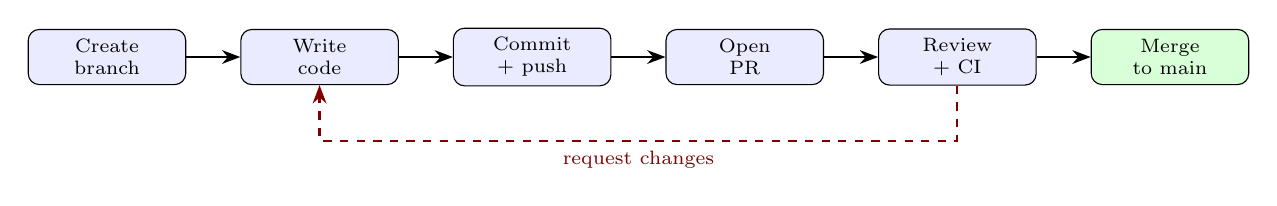
\begin{tikzpicture}[
      box/.style={draw, rounded corners, fill=blue!8, minimum width=2cm, minimum height=0.7cm, align=center, font=\scriptsize},
      arr/.style={->, thick, >=Stealth}
    ]
      \node[box] (branch) at (0,0)     {Create\\branch};
      \node[box] (code)   at (2.7,0)   {Write\\code};
      \node[box] (commit) at (5.4,0)   {Commit\\+ push};
      \node[box] (pr)     at (8.1,0)   {Open\\PR};
      \node[box] (review) at (10.8,0)  {Review\\+ CI};
      \node[box, fill=green!15] (merge) at (13.5,0) {Merge\\to main};
      \draw[arr] (branch)--(code);
      \draw[arr] (code)--(commit);
      \draw[arr] (commit)--(pr);
      \draw[arr] (pr)--(review);
      \draw[arr] (review)--(merge);
      % feedback loop
      \draw[arr, dashed, red!50!black] (review.south) -- ++(0,-0.7) -| node[below, near start, font=\scriptsize\color{red!50!black}] {request changes} (code.south);
    \end{tikzpicture}
  \end{center}

  \vspace{0.5em}
  \textbf{After merge:}
  \begin{itemize}
    \item Delete the feature branch (GitHub can auto-delete).
    \item Pull \texttt{main} locally: \texttt{git checkout main \&\& git pull}.
    \item Start the next branch from the updated \texttt{main}.
  \end{itemize}
\end{frame}

% ============================================================
\section{Best Practices}
% ============================================================

\begin{frame}{The Golden Rules}
  \begin{enumerate}
    \item \textbf{Never push directly to \texttt{main}.} \emph{Always} use a branch + PR.
    \item \textbf{Commit often, push daily.} Small, logical, atomic commits.
    \item \textbf{Pull before you push} to avoid unnecessary conflicts.
    \item \textbf{One PR = one concern.} Don't mix a bug fix with a new feature.
    \item \textbf{Protect \texttt{main}} with branch protection rules.
    \item \textbf{Delete merged branches} --- keep the branch list clean.
    \item \textbf{Use \texttt{.gitignore}} --- don't track build artefacts, data, or secrets.
    \item \textbf{Tag releases:} \texttt{git tag -a v1.0 -m "Submission version"}
    \item \textbf{Never commit secrets} (passwords, API keys, \texttt{.env} files).
    \item \textbf{Don't commit large binaries} --- use Git LFS if needed.
  \end{enumerate}
\end{frame}

\begin{frame}{Branch Naming --- Summary}
  \begin{table}
    \centering
    \begin{tabular}{@{} l l @{}}
      \toprule
      \textbf{Do} & \textbf{Don't} \\
      \midrule
      \texttt{feature/add-k-epsilon}     & \texttt{new-stuff} \\
      \texttt{fix/42-inlet-nan}          & \texttt{fix} \\
      \texttt{docs/update-install-guide} & \texttt{branch1} \\
      \texttt{refactor/solver-module}    & \texttt{muaaz-changes} \\
      \texttt{exp/gpu-acceleration}      & \texttt{test123} \\
      \bottomrule
    \end{tabular}
  \end{table}

  \vspace{0.5em}
  \textbf{Format:} \texttt{type/short-hyphenated-description}\\
  \textbf{Prefixes:} \texttt{feature/}, \texttt{fix/}, \texttt{docs/}, \texttt{refactor/}, \texttt{test/}, \texttt{chore/}, \texttt{exp/}\\
  \textbf{Optionally include issue number:} \texttt{fix/42-nan-at-outlet}
\end{frame}

\begin{frame}{Commit Message Convention}
  A widely adopted format:

  \vspace{0.5em}
  \texttt{<type>: <short description>}

  \vspace{0.5em}
  \begin{table}
    \centering
    \begin{tabular}{@{} l l l @{}}
      \toprule
      \textbf{Type} & \textbf{Meaning} & \textbf{Example} \\
      \midrule
      \texttt{feat}     & New feature           & \texttt{feat: add k-epsilon turbulence model} \\
      \texttt{fix}      & Bug fix               & \texttt{fix: correct wall boundary condition} \\
      \texttt{docs}     & Documentation only    & \texttt{docs: update README with install steps} \\
      \texttt{refactor} & No behaviour change   & \texttt{refactor: extract mesh class} \\
      \texttt{test}     & Adding / fixing tests & \texttt{test: add mesh convergence tests} \\
      \texttt{chore}    & Build, tooling, deps  & \texttt{chore: upgrade numpy to 2.0} \\
      \bottomrule
    \end{tabular}
  \end{table}

  \vspace{0.3em}
  \textbf{Good message:} \texttt{fix: prevent NaN at outlet boundary} \checkmark \\
  \textbf{Bad messages:} \texttt{stuff}, \texttt{update}, \texttt{fix bug}, \texttt{wip} \texttimes
\end{frame}

\begin{frame}{PR Checklist --- Before You Hit ``Create''}
  Use this as a mental (or actual) checklist for every PR:

  \vspace{0.5em}
  \begin{enumerate}
    \item[\checkmark] \textbf{Branch} is named correctly (\texttt{type/description}).
    \item[\checkmark] \textbf{Title} is clear and in imperative mood.
    \item[\checkmark] \textbf{Description} explains \emph{what} and \emph{why}, links the issue.
    \item[\checkmark] \textbf{Scope is small} --- one feature or one fix per PR.
    \item[\checkmark] \textbf{Tests pass} locally before pushing.
    \item[\checkmark] \textbf{No unrelated changes} (formatting, whitespace, other files).
    \item[\checkmark] \textbf{Self-review:} read your own diff before requesting review.
    \item[\checkmark] \textbf{Docs updated} if behaviour or API changed.
    \item[\checkmark] \textbf{No secrets or large files} committed.
  \end{enumerate}

  \vspace{0.5em}
  \begin{block}{Tip}
    Many teams put this checklist in a \textbf{PR template} (\texttt{.github/PULL\_REQUEST\_TEMPLATE.md}) so it auto-fills every time.
  \end{block}
\end{frame}

% ============================================================
\section{Repository Essentials: README, LICENCE \& .gitignore}
% ============================================================

\begin{frame}{Why Every Repo Needs a README}
  The \texttt{README.md} is the \textbf{front door} of your project --- it's the first thing anyone sees on GitHub.

  \vspace{0.3em}
  \textbf{Without a README:}
  \begin{itemize}
    \item Collaborators don't know how to install or run your code.
    \item Future-you (6 months later) won't remember what this repo does.
    \item Nobody will use or cite your work --- they can't figure it out.
    \item Your supervisor opens the repo and sees\ldots a wall of files.
  \end{itemize}

  \vspace{0.3em}
  \textbf{With a good README:}
  \begin{itemize}
    \item Anyone can understand, install, and run the project in minutes.
    \item It serves as lightweight documentation that lives with the code.
    \item It signals professionalism and care --- people trust well-documented code.
    \item GitHub renders it automatically below the file listing.
  \end{itemize}

  \vspace{0.3em}
  \begin{alertblock}{Rule}
    \textbf{No README = the repo doesn't exist} to anyone but you. If someone needs more than 30 seconds to figure out what your project does, the README has failed.
  \end{alertblock}
\end{frame}

\begin{frame}[fragile]{Writing a Good README}
  \textbf{Essential sections} (in order):

  \vspace{0.3em}
  \begin{enumerate}
    \item \textbf{Title \& one-line description} --- what is this?
    \item \textbf{Installation / setup} --- how do I get it running?
    \item \textbf{Usage} --- show me a quick example.
    \item \textbf{Project structure} --- what's in each folder?
    \item \textbf{Contributing} --- how can others help? (if applicable)
    \item \textbf{Licence} --- what am I allowed to do with this code?
    \item \textbf{Citation} --- how should others cite this work? (academic projects)
  \end{enumerate}

  \vspace{0.3em}
  \begin{lstlisting}[language={}, basicstyle=\ttfamily\tiny, title={Minimal README skeleton}]
# Project Name

One-sentence description of what this project does.

## Installation
```bash
git clone https://github.com/user/project.git
cd project
pip install -r requirements.txt
```

## Usage
```bash
python src/main.py --input data/mesh.vtk
```

## Licence
MIT --- see [LICENSE](LICENSE).
  \end{lstlisting}
\end{frame}

\begin{frame}{README Best Practices}
  \begin{columns}[T]
    \begin{column}{0.48\textwidth}
      \textbf{Do:}
      \begin{itemize}
        \item Start with what the project \emph{does}, not how.
        \item Include a working ``quick start'' that a newcomer can copy--paste.
        \item List dependencies and versions explicitly.
        \item Add badges (CI status, licence, Python version).
        \item Keep it up to date --- stale docs are worse than no docs.
        \item For academic code: include a citation block (BibTeX).
      \end{itemize}
    \end{column}
    \begin{column}{0.48\textwidth}
      \textbf{Don't:}
      \begin{itemize}
        \item Leave the default GitHub-generated one-liner.
        \item Write a novel --- keep it scannable.
        \item Assume the reader knows your project.
        \item Put detailed API docs in the README --- link to separate docs instead.
        \item Forget to mention the licence.
      \end{itemize}

      \vspace{0.5em}
      \textbf{Tip:} GitHub supports adding a \texttt{CITATION.cff} file that generates a ``Cite this repository'' button.
    \end{column}
  \end{columns}
\end{frame}

\begin{frame}{Why Every Repo Needs a LICENCE}
  \textbf{No licence = no permission.}

  \vspace{0.3em}
  Under copyright law, code without a licence is \textbf{all rights reserved} by default. That means nobody can legally use, modify, or distribute your code --- even if it's public on GitHub.

  \vspace{0.5em}
  \textbf{A licence:}
  \begin{itemize}
    \item Tells others \emph{exactly} what they can and can't do with your code.
    \item Protects you from liability (most licences include a warranty disclaimer).
    \item Is \textbf{required} by many journals and funders for reproducible research.
    \item Takes 30 seconds to add --- GitHub offers a licence picker when creating a repo.
  \end{itemize}

  \vspace{0.5em}
  \begin{alertblock}{Academic code}
    If you publish a paper and share the code on GitHub without a licence, \textbf{nobody can legally reproduce your results}. This defeats the purpose of open science.
  \end{alertblock}
\end{frame}

\begin{frame}{Choosing a Licence}
  \begin{table}
    \centering
    \begin{tabular}{@{} l p{5.5cm} l @{}}
      \toprule
      \textbf{Licence} & \textbf{What it allows} & \textbf{Use when} \\
      \midrule
      \textbf{MIT} &
        Do anything; keep the copyright notice. &
        Maximum freedom \\
      \textbf{Apache 2.0} &
        Like MIT + explicit patent grant. &
        Patent-sensitive code \\
      \textbf{GPL v3} &
        Modifications must also be open source. &
        You want copyleft \\
      \textbf{BSD 3-Clause} &
        Like MIT; can't use your name to endorse. &
        Academic tradition \\
      \textbf{CC BY 4.0} &
        For non-code (docs, data, figures). &
        Data \& creative works \\
      \bottomrule
    \end{tabular}
  \end{table}

  \vspace{0.3em}
  \textbf{How to add a licence:}
  \begin{itemize}
    \item GitHub: \textbf{Add file} $\to$ type \texttt{LICENSE} $\to$ \textbf{Choose a licence template}.
    \item Or: \url{https://choosealicense.com} --- answer a few questions, copy the text.
    \item The file must be in the \textbf{root} of your repo, named \texttt{LICENSE} or \texttt{LICENSE.md}.
  \end{itemize}

  \vspace{0.3em}
  \begin{block}{When in doubt}
    \textbf{MIT} is the most popular choice for academic and open-source code. It's short, permissive, and well-understood.
  \end{block}
\end{frame}

\begin{frame}[fragile]{Why Every Repo Needs a .gitignore}
  Git tracks \emph{everything} you \texttt{git add}. Without a \texttt{.gitignore}, you'll accidentally commit:

  \vspace{0.3em}
  \begin{columns}[T]
    \begin{column}{0.48\textwidth}
      \textbf{Things that should never be tracked:}
      \begin{itemize}
        \item Build artefacts (\texttt{*.pyc}, \texttt{\_\_pycache\_\_/}, \texttt{build/})
        \item IDE settings (\texttt{.vscode/}, \texttt{.idea/})
        \item OS junk (\texttt{.DS\_Store}, \texttt{Thumbs.db})
        \item Secrets (\texttt{.env}, \texttt{*.key}, \texttt{*.pem})
        \item Large data/output files (\texttt{*.vtk}, \texttt{*.h5})
        \item Virtual environments (\texttt{venv/}, \texttt{.venv/})
        \item \LaTeX{} aux files (\texttt{*.aux}, \texttt{*.log})
      \end{itemize}
    \end{column}
    \begin{column}{0.48\textwidth}
      \textbf{Why this matters:}
      \begin{itemize}
        \item Bloats the repo --- cloning takes forever.
        \item Secrets on GitHub = security breach.
        \item Merge conflicts in generated files waste time.
        \item Reviewers see noise instead of real changes.
        \item Some files are machine-specific and break on other systems.
      \end{itemize}
    \end{column}
  \end{columns}

  \vspace{0.5em}
  \begin{alertblock}{Once tracked, always tracked}
    \texttt{.gitignore} only prevents \emph{new} files from being tracked. If you've already committed a file, adding it to \texttt{.gitignore} won't remove it. You must also run:\\
    \texttt{git rm --cached <file>}
  \end{alertblock}
\end{frame}

\begin{frame}[fragile]{Writing a Good .gitignore}
  \textbf{Syntax:}
  \begin{lstlisting}[language={}, basicstyle=\ttfamily\scriptsize]
# Comment
*.pyc              # ignore all .pyc files (anywhere)
__pycache__/       # ignore directory
.env               # ignore specific file
build/             # ignore build output
!important.pyc     # exception --- DO track this one
data/*.csv         # ignore CSVs only in data/
**/logs/           # ignore logs/ at any depth
  \end{lstlisting}

  \vspace{0.3em}
  \textbf{Don't write one from scratch.} Use a template:
  \begin{itemize}
    \item GitHub: when creating a repo $\to$ \textbf{Add .gitignore} $\to$ select language.
    \item \url{https://gitignore.io} --- generates a \texttt{.gitignore} for any combination of languages, IDEs, and OSes.
    \item \texttt{gh repo create} with \texttt{--gitignore Python} (or any template name).
  \end{itemize}

  \vspace{0.3em}
  \begin{block}{Pro tip: global gitignore}
    OS and editor files (\texttt{.DS\_Store}, \texttt{.vscode/}) belong in a \textbf{global} gitignore, not in every repo:
    \begin{lstlisting}[language=bash, basicstyle=\ttfamily\scriptsize]
git config --global core.excludesFile ~/.gitignore_global
    \end{lstlisting}
  \end{block}
\end{frame}

\begin{frame}{The First Commit Checklist}
  Before writing any code, every new repo should have these three files:

  \vspace{0.5em}
  \begin{table}
    \centering
    \begin{tabular}{@{} l l p{7cm} @{}}
      \toprule
      \textbf{File} & \textbf{Purpose} & \textbf{Action} \\
      \midrule
      \texttt{README.md} &
        What this project is and how to use it &
        Write at least a title, one-line description, and install instructions. \\
      \texttt{LICENSE} &
        Legal permissions for your code &
        Pick MIT (or appropriate) via GitHub's template picker. \\
      \texttt{.gitignore} &
        Prevent junk from being tracked &
        Generate from \texttt{gitignore.io} for your language + IDE + OS. \\
      \bottomrule
    \end{tabular}
  \end{table}

  \vspace{0.5em}
  \begin{block}{Make it automatic}
    \texttt{gh repo create my-project --public --clone --license mit --gitignore Python --add-readme}\\[3pt]
    One command, all three files, done.
  \end{block}
\end{frame}

% ============================================================
\section{Hands-On Exercises}
% ============================================================

\begin{frame}{Exercises Overview}
  Open the \texttt{exercises/} folder in this repository.

  \begin{enumerate}
    \item \textbf{01-first-repo} --- init, add, commit, push, \texttt{.gitignore}.
    \item \textbf{02-branching-merging} --- branches, checkout, merge.
    \item \textbf{03-collaboration} --- fork, clone, pull request.
    \item \textbf{04-conflict-resolution} --- create and resolve a merge conflict.
    \item \textbf{05-gh-cli} --- use \texttt{gh} to create repos, PRs, and issues.
  \end{enumerate}

  \vspace{0.5em}
  Each folder has a \texttt{README.md} with step-by-step instructions and challenges.

  \vspace{0.5em}
  \begin{block}{Bonus}
    Try the \texttt{sample-project/} folder --- a small Python project you can use to practise the full workflow: branch, edit code, commit, push, open a PR.
  \end{block}
\end{frame}

% ============================================================
\section{Summary \& Resources}
% ============================================================

\begin{frame}{Summary}
  \begin{table}
    \centering
    \begin{tabular}{@{} l p{10cm} @{}}
      \toprule
      \textbf{Topic} & \textbf{Key takeaway} \\
      \midrule
      Terminal / UI / \texttt{gh} / VS Code & Four tools, one repo. Learn the terminal first, then add the GUI tools. \\
      Authentication & SSH keys for daily use; \texttt{gh auth login} for a quick start. \\
      Branching  & Never commit directly to \texttt{main}. One branch per task, named \texttt{type/description}. \\
      Forking    & Fork when you don't have write access. Branch inside the fork, submit a PR upstream. \\
      Pull Requests & Every change goes through a PR --- small, focused, reviewed, tested. \\
      Branch protection & Enforce PRs + reviews + CI on \texttt{main}. Even solo projects benefit. \\
      Repo essentials & Every repo starts with three files: \texttt{README.md}, \texttt{LICENSE}, and \texttt{.gitignore}. No exceptions. \\
      \bottomrule
    \end{tabular}
  \end{table}
\end{frame}

\begin{frame}{Resources}
  \textbf{Official:}
  \begin{itemize}
    \item \href{https://git-scm.com/book/en/v2}{Pro Git Book} (free, comprehensive)
    \item \href{https://docs.github.com}{GitHub Docs}
    \item \href{https://cli.github.com/manual/}{GitHub CLI Manual}
  \end{itemize}

  \textbf{Interactive:}
  \begin{itemize}
    \item \href{https://learngitbranching.js.org/}{Learn Git Branching} --- visual, gamified
    \item \href{https://github.com/jlord/git-it-electron}{git-it} --- desktop tutorial
    \item \href{https://ohmygit.org/}{Oh My Git!} --- card game
  \end{itemize}

  \textbf{Cheat sheets:}
  \begin{itemize}
    \item \href{https://education.github.com/git-cheat-sheet-education.pdf}{GitHub's official cheat sheet}
    \item The \texttt{cheatsheet/} folder in this repo
  \end{itemize}

  \vspace{1em}
  \centering
  \Large\textbf{Questions?}

  \vspace{0.5em}
  \normalsize
  \href{mailto:muaaz.bhamjee@up.ac.za}{muaaz.bhamjee@up.ac.za}
\end{frame}

\end{document}
